Consider the following activity diagram:



\begin{centering}
\includegraphics[min width=0.4\textwidth=0.6\textwidth,min height=0.4\textwidth=0.6\textwidth,keepaspectratio,max width=0.9\textwidth,max height=0.9\textwidth]{70/Diagram.pdf}\end{centering}

Consider the following Petri net as translation of this activity diagram:



\begin{centering}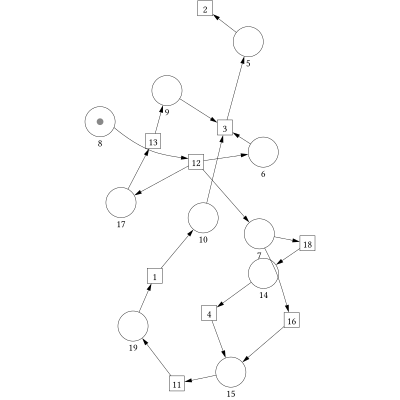
\includegraphics[min width=0.4\textwidth=0.6\textwidth,min height=0.4\textwidth=0.6\textwidth,keepaspectratio,max width=0.9\textwidth,max height=0.9\textwidth]{70/petricff5a4044ef80069aea069d6f718e4f1b1e9e2d0fd37f570e68155927b33e2ba11014.pdf}\end{centering}

State each matching of action node and Petri net node, each matching of object node and Petri net node, the Petri net nodes per other element kind, as well as all auxiliary places and auxiliary transitions in the Petri net.

To do this, enter your answer as in the following example:
\begin{minted}{text}
MatchPetriSolution {actionNodes = [("A",1),("B",2)], objectNodes = [("C",3),("D",4)], decisionNodes = [5,7], mergeNodes = [6,8], forks = [10], joins = [11], initialNodes = [12], activityFinalNodes = [16], flowFinalNodes = [], auxiliaryPetriNodes = [13,14,15]}
\end{minted}

In this example, the action nodes ``A'' and ``B'' are matched with the Petri net nodes 1 and 2, the Petri net nodes 5 and 7 correspond to decision nodes, the Petri net nodes 13, 14 and 15 are auxiliary places or auxiliary transitions, the Petri net node 16 corresponds to an activity final node, and no Petri net node corresponds to a flow final node.

Hint on the translation to a Petri net: For final nodes no additional places are introduced. They are realised in a way that a token is consumed, i.e. disappears from the net at that position. If an additional transition is required to realise this behavior at a position in the diagram where there is a final node, this transition does not count as auxiliary node.

